% Created 2023-05-13 Sat 15:06
% Intended LaTeX compiler: pdflatex
\documentclass[9pt, b5paper]{article}
\usepackage{xeCJK}
\usepackage[T1]{fontenc}
\usepackage{bera}
\usepackage[scaled]{beraserif}
\usepackage[scaled]{berasans}
\usepackage[scaled]{beramono}
\usepackage[cache=false]{minted}
\usepackage{xltxtra}
\usepackage{graphicx}
\usepackage{xcolor}
\usepackage{multirow}
\usepackage{multicol}
\usepackage{float}
\usepackage{textcomp}
\usepackage{algorithm}
\usepackage{algorithmic}
\usepackage{latexsym}
\usepackage{natbib}
\usepackage{geometry}
\geometry{left=1.2cm,right=1.2cm,top=1.5cm,bottom=1.2cm}
\usepackage[xetex,colorlinks=true,CJKbookmarks=true,linkcolor=blue,urlcolor=blue,menucolor=blue]{hyperref}
\newminted{common-lisp}{fontsize=\footnotesize} 
\author{deepwaterooo}
\date{\today}
\title{ET 框架学习笔记--自己需要这样一个总结文档来帮助总结与急速重构自己的游戏}
\hypersetup{
 pdfauthor={deepwaterooo},
 pdftitle={ET 框架学习笔记--自己需要这样一个总结文档来帮助总结与急速重构自己的游戏},
 pdfkeywords={},
 pdfsubject={},
 pdfcreator={Emacs 28.2 (Org mode 9.5.5)}, 
 pdflang={English}}
\begin{document}

\maketitle
\tableofcontents


\section{UI 上的事件驱动系统:}
\label{sec:orgc536f4f}
\subsection{EventType}
\label{sec:orgb952841}
\begin{minted}[fontsize=\scriptsize,linenos=false]{csharp}
namespace EventType {
    public struct SceneChangeStart {
    }
    public struct SceneChangeFinish {
    }

    public struct AfterCreateClientScene {
    }
    public struct AfterCreateCurrentScene {
    }

    public struct AppStartInitFinish {
    }
    public struct LoginFinish {
    }
    // public struct EnterMapFinish {
    public struct EnterRoomFinish {
    }
    public struct AfterUnitCreate {
        public Unit Unit;
    }
}
\end{minted}
\subsection{由 AppStartInitFinish 事件所触发的 CreateLoginUI}
\label{sec:org63a641d}
\begin{minted}[fontsize=\scriptsize,linenos=false]{csharp}
[Event(SceneType.Client)] // ET 事件系统的工具,标签系
public class AppStartInitFinish_CreateLoginUI: AEvent<EventType.AppStartInitFinish> {
\end{minted}
\subsection{由 LoginFinish 事件所触发的 CreateLobbyUI}
\label{sec:org23dcdd2}
\begin{minted}[fontsize=\scriptsize,linenos=false]{csharp}
[Event(SceneType.Client)]
public class LoginFinish_CreateLobbyUI: AEvent<EventType.LoginFinish> {
\end{minted}
\begin{itemize}
\item 这些是原示范框架都已经完成了的,我只需要添加剩余的逻辑。
\end{itemize}
\subsection{现游戏项目 ET7 里的主要适配:由原UI 上的组件系统,手动组件添加移除,更改为UI 上的事件驱动系统的事件定义,注册,与工厂生成系?}
\label{sec:orga0910d2}
\begin{itemize}
\item 就是说,接下来游戏里的主要逻辑,也将变成如此一个个不同的自定义事件,来驱动UI 上的各种回调。【爱表哥,爱生活!!!活宝妹就是一定要嫁给亲爱的表哥!!!】
\item UI 界面上的按钮点击要如何处理呢,新框架里,找个例子看看,点【进入地图】看看: \textbf{全部变成了Helper 帮助类}
\end{itemize}

\section{Helper 类的总结: 【但凡点击回调方法,就变成Helper 类!】为什么就变成了这么一个个的帮助类呢?}
\label{sec:orgdd51a96}
\subsection{LoginHelper.cs}
\label{sec:org269e354}
\begin{minted}[fontsize=\scriptsize,linenos=false]{csharp}
public static class LoginHelper {
public static async ETTask Login(Scene clientScene, string account, string password) {
    try {
        // 创建一个ETModel层的Session
        clientScene.RemoveComponent<RouterAddressComponent>();
        // 获取路由跟realmDispatcher地址
        RouterAddressComponent routerAddressComponent = clientScene.GetComponent<RouterAddressComponent>();
        if (routerAddressComponent == null) {
            routerAddressComponent = clientScene.AddComponent<RouterAddressComponent, string, int>(ConstValue.RouterHttpHost, ConstValue.RouterHttpPort);
            await routerAddressComponent.Init();

            clientScene.AddComponent<NetClientComponent, AddressFamily>(routerAddressComponent.RouterManagerIPAddress.AddressFamily);
        }
        IPEndPoint realmAddress = routerAddressComponent.GetRealmAddress(account);

        R2C_Login r2CLogin;
        using (Session session = await RouterHelper.CreateRouterSession(clientScene, realmAddress)) {
            r2CLogin = (R2C_Login) await session.Call(new C2R_Login() { Account = account, Password = password });
        }
        // 创建一个gate Session,并且保存到SessionComponent中: 与网关服的会话框。主要负责用户下线后会话框的自动移除销毁
        Session gateSession = await RouterHelper.CreateRouterSession(clientScene, NetworkHelper.ToIPEndPoint(r2CLogin.Address));
        clientScene.AddComponent<SessionComponent>().Session = gateSession;

        G2C_LoginGate g2CLoginGate = (G2C_LoginGate)await gateSession.Call(
            new C2G_LoginGate() { Key = r2CLogin.Key, GateId = r2CLogin.GateId});
        Log.Debug("登陆gate成功!");
        await EventSystem.Instance.PublishAsync(clientScene, new EventType.LoginFinish());
    }
    catch (Exception e) {
        Log.Error(e);
    }
} 
}
\end{minted}
\subsection{EnterRoomHelper.cs}
\label{sec:orgcb53723}
\begin{itemize}
\item 这里需要注意的是:原项目里面还是保留了C2G\_EnterMap 消息的。分两块查看一下:
\begin{itemize}
\item 可以先去查一下,斗地主里是如何【开始匹配】的
\item ET 7 框架里,服务器是如何处理消息的,变成了不同的 \textbf{场景类型:SceneType, 由不同场景,也就是不同的专职服务器来处理各种逻辑功能块的消息}
\begin{itemize}
\item 仍然是 \textbf{标签系的消息处理器}: 因为先前的不同服变成了现在的不同场景,分场景(先前的不同服)来定义消息处理器,以处理当前场景(特定功能逻辑服)下的消息,如匹配服的消息。
\end{itemize}
\item \textbf{如果每个按钮的回调:都单独一个类,不成了海量回调类了?}
\item 老版本:斗地主里,进入地图的参考 \textbf{【ET】里,就要去找,如何处理这些组件的?}
\end{itemize}
\end{itemize}
\begin{minted}[fontsize=\scriptsize,linenos=false]{csharp}
// public static class EnterMapHelper {
public static class EnterRoomHelper {

// 进拖拉拉机房:异步过程,需要与房间服交互的. 【房间服】:
// 【C2G_EnterRoom】:消息也改下
public static async ETTask EnterRoomAsync(Scene clientScene) {
    try {
        G2C_EnterMap g2CEnterMap = await clientScene.GetComponent<SessionComponent>().Session.Call(new C2G_EnterMap()) as G2C_EnterMap;
        clientScene.GetComponent<PlayerComponent>().MyId = g2CEnterMap.MyId;

        // 等待场景切换完成
        await clientScene.GetComponent<ObjectWait>().Wait<Wait_SceneChangeFinish>();

        // EventSystem.Instance.Publish(clientScene, new EventType.EnterMapFinish());
        EventSystem.Instance.Publish(clientScene, new EventType.EnterRoomFinish()); // 这个,再去找下,谁在订阅这个事件,如何带动游戏开启的状态?

        // // 老版本:斗地主里,进入地图的参考【ET7】里,就要去找,如何处理这些组件的?
        // Game.Scene.AddComponent<OperaComponent>();
        // Game.Scene.GetComponent<UIComponent>().Remove(UIType.UILobby);
    }
    catch (Exception e) {
        Log.Error(e);
    }    
}
}
\end{minted}
\begin{itemize}
\item 一个服务器端的消息处理器供自己参考:【分场景的消息处理器,仍使用标签系】
\begin{minted}[fontsize=\scriptsize,linenos=false]{csharp}
[MessageHandler(SceneType.Client)]
public class M2C_CreateMyUnitHandler : AMHandler<M2C_CreateMyUnit> {
    protected override async ETTask Run(Session session, M2C_CreateMyUnit message) {
        // 通知场景切换协程继续往下走
        session.DomainScene().GetComponent<ObjectWait>().Notify(new Wait_CreateMyUnit() {Message = message});
        await ETTask.CompletedTask;
    }
}
\end{minted}
\item 再来一个场景切换开始事件的:【任何时候,活宝妹就是一定要嫁给亲爱的表哥!!!】
\begin{minted}[fontsize=\scriptsize,linenos=false]{csharp}
// 这个比较喜欢:场景切换, 先前不同功能定义的服,切换开始,可以做点什么?切换结束,可以做点什么?全成事件触发机制。
[Event(SceneType.Client)]
public class SceneChangeStart_AddComponent: AEvent<EventType.SceneChangeStart> {

    protected override async ETTask Run(Scene scene, EventType.SceneChangeStart args) {
        Scene currentScene = scene.CurrentScene();
            
        // 加载场景资源
        await ResourcesComponent.Instance.LoadBundleAsync($"{currentScene.Name}.unity3d");
        // 切换到map场景
        await SceneManager.LoadSceneAsync(currentScene.Name);
            
        currentScene.AddComponent<OperaComponent>();
    }
}
\end{minted}
\end{itemize}

\section{服务器类型 AppType, 变成为路由系统 RouterAddressComponent}
\label{sec:orgf549bbd}
\begin{itemize}
\item 应用的类型,新框架里有如下几种
\end{itemize}
\begin{minted}[fontsize=\scriptsize,linenos=false]{csharp}
public enum AppType {
    Server,
    Watcher, // 每台物理机一个守护进程,用来启动该物理机上的所有进程
    GameTool,
    ExcelExporter,
    Proto2CS,
    BenchmarkClient,
    BenchmarkServer,
}
\end{minted}
\begin{itemize}
\item 但是场景的类型,保留了先前的:不是还要添加Match 匹配服?
\begin{itemize}
\item 可以再找具体的例子来看
\end{itemize}
\begin{minted}[fontsize=\scriptsize,linenos=false]{csharp}
public enum SceneType {
    None = -1,
    Process = 0,
    Manager = 1,
    Realm = 2, // 【注册登录服】
    Gate = 3,  // 【网关服】
    Http = 4,
    Location = 5, // 【地址服】
    Map = 6,      // 【地图服】
    Router = 7,
    RouterManager = 8,
    Robot = 9,
    BenchmarkClient = 10,
    BenchmarkServer = 11,
    Benchmark = 12,
    // 客户端Model层
    Client = 31,
    Current = 34,
}
\end{minted}
\end{itemize}
\section{辅助事理:框架里的各系统}
\label{sec:orga552b99}
\subsection{标签系: 标签系统重构了,现分为几个类型}
\label{sec:org3314584}
\subsubsection{ComponentOfAttribute : Attribute}
\label{sec:org8a176b4}
\begin{minted}[fontsize=\scriptsize,linenos=false]{csharp}
// 组件类父级实体类型约束
// 父级实体类型唯一的 标记指定父级实体类型【ComponentOf(typeof(parentType)】
// 不唯一则标记【ComponentOf]
[AttributeUsage(AttributeTargets.Class)]
public class ComponentOfAttribute : Attribute {
    public Type Type;
    public ComponentOfAttribute(Type type = null) {
        this.Type = type;
    }
}
\end{minted}
\subsubsection{ComponentView: MonoBehaviour}
\label{sec:orgbfd9504}
\begin{minted}[fontsize=\scriptsize,linenos=false]{csharp}
public class ComponentView: MonoBehaviour {
    public Entity Component {
        get;
        set;
    }
}
\end{minted}
\textbf{*}

\section{整个框架: ET 7.2 + YooAssets + luban + FairGUI}
\label{sec:org4bb3278}
\begin{itemize}
\item 整个框架的场景节点如下
\end{itemize}

\begin{center}
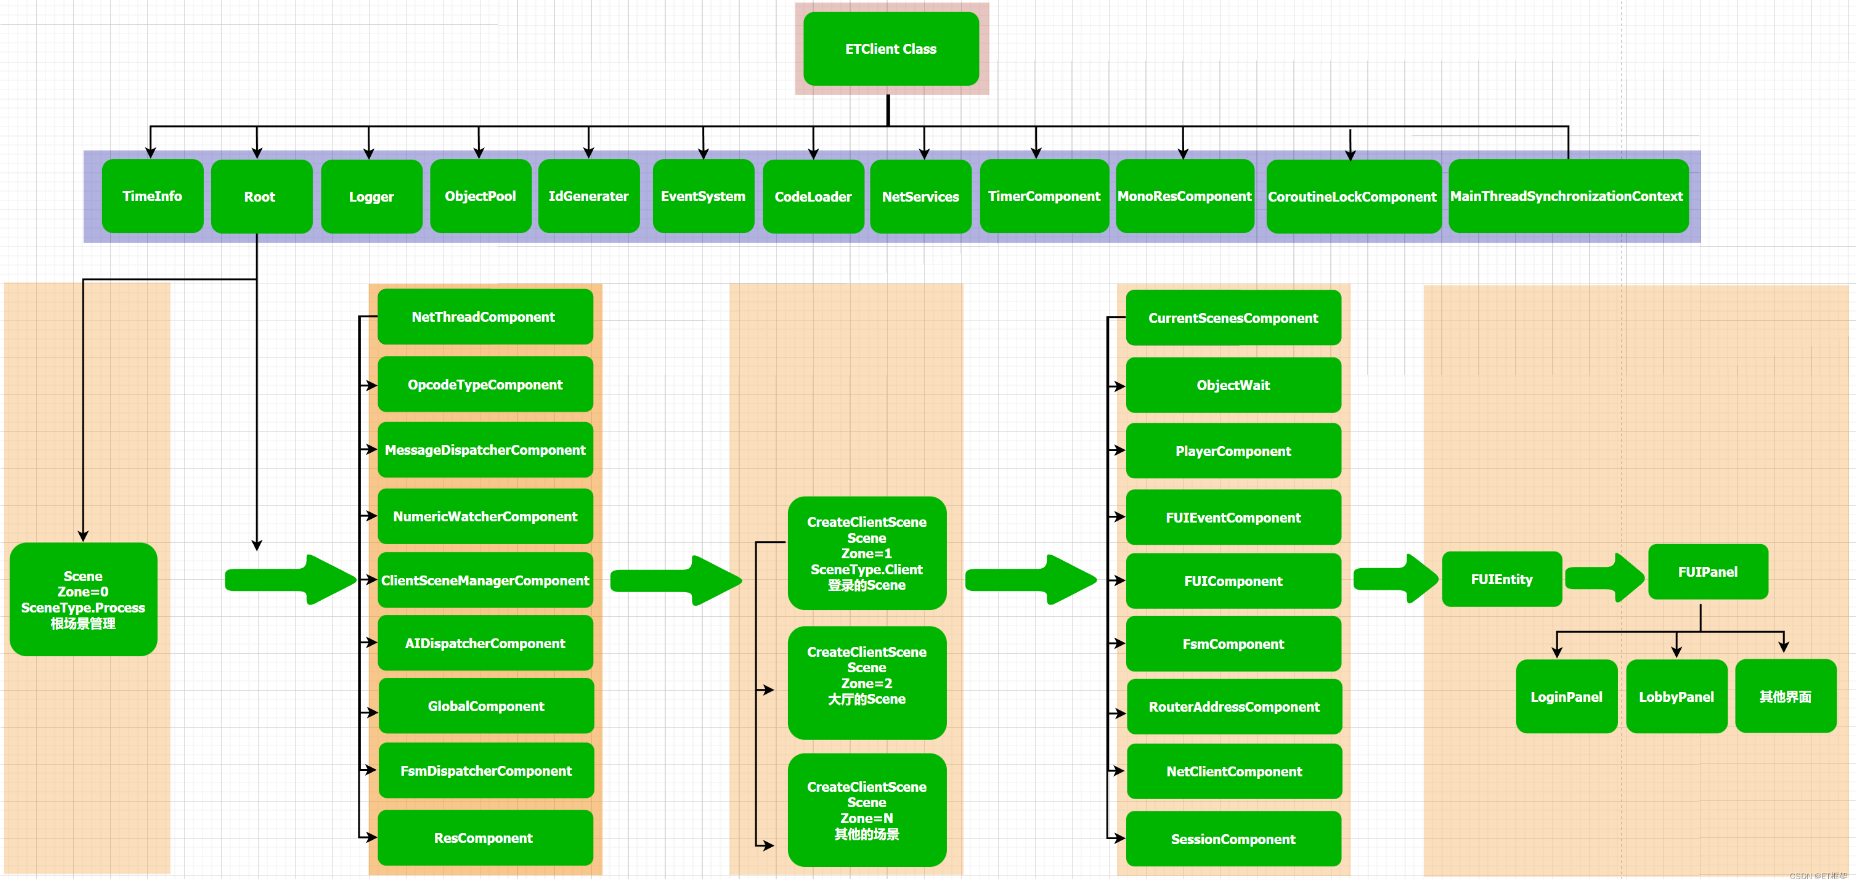
\includegraphics[width=.9\linewidth]{./pic/ET_20230512_143227.png}
\end{center}

\section{写在最后:反而是自己每天查看一再更新的}
\label{sec:org761824b}
\begin{itemize}
\item 因为感觉还是不曾系统性地读ET7 的源码,或者说有效阅读,因为没有带着实际问题的看源码,感觉都不叫看读源码呀。这里会记自己的感觉需要赶快查看的地方。
\item 【ET 框架的整体架构】:感觉把握不够。常常命名空间分不清。要把这个大的框架,比较高层面的架构再好好看下
\item 然后就是对自顶向下的不同层级场景,所需要的主要的不同组件,分不清,仍需要再熟悉一下源码
\item 错太多,其它难点儿的还不熟悉源码,就把所有的【Proto 消息】先生成出来,能去掉一半错误。今天晚上至少可以把这个全部解决掉
\begin{itemize}
\item 【问题】:某些消息,还分不清是内网还是外网消息,暂时先放一下,到时再改
\item 【问题】:上次那个ET-EUI 框架的时候,曾经出现过 opcode 不对应,也就是说,我现在生成的进程间消息,有可能还是会存在服务器码与客户端码不对应,这个完备的框架,这次应该不至于吧?
\end{itemize}
\item 改 compile-error 时,不知道为佳么,感觉 mac 下的VSC 比 windows 好用,用那个先改下
\end{itemize}

\section{现在的修改内容,记忆}
\label{sec:org503b1ba}
\begin{itemize}
\item UILobbyComponent 里三个按钮的回调:这里面还有好几个错误。把这个弄完了,出错在更晚的地方的话,这个界面就可以加载完整了。。
\end{itemize}
\begin{minted}[fontsize=\scriptsize,linenos=false]{csharp}
// 获取玩家数据: 按说应该是注册登录服的逻辑,或者是数据库服存放着用户信息,都是通过Gate中转
        long userId = ClientComponent.Instance.LocalPlayer.UserID; // 【ClientComponent】:组件被重构掉了,去找相应的替换
        C2G_GetUserInfo_Req c2G_GetUserInfo_Req = new C2G_GetUserInfo_Req() { UserID = userId }; // 去从网关服拿玩家信息
        G2C_GetUserInfo_Ack g2C_GetUserInfo_Ack = await SessionComponent.Instance.Session.Call(c2G_GetUserInfo_Req) as G2C_GetUserInfo_Ack;
        // 显示用户信息
        rc.Get<GameObject>("NickName").GetComponent<Text>().text = g2C_GetUserInfo_Ack.NickName;
        rc.Get<GameObject>("Money").GetComponent<Text>().text = g2C_GetUserInfo_Ack.Money.ToString();                
    }
}
// 【回调:】自定义三个按钮的回调。这些个过程流程,就主要参考,同框架的斗地主游戏
public static async ETTask matchRoom(this UILobbyComponent self) { // 通过网关服中转,请求匹配服为给匹配一个房间四人桌
    try {
        // 发送开始匹配消息
        C2G_StartMatch_Req c2G_StartMatch_Req = new C2G_StartMatch_Req();
        G2C_StartMatch_Ack g2C_StartMatch_Ack = await SessionComponent.Instance.Session.Call(c2G_StartMatch_Req) as G2C_StartMatch_Ack; // 这里去看下服务器的处理逻辑
        // // 暫时跳过这步
        // if (g2C_StartMatch_Ack.Error == ErrorCode.ERR_UserMoneyLessError) {
        //     Log.Error("余额不足"); // 就是说,当且仅当余额不足的时候才会出这个错误?
        //     return;
        // }
        // 匹配成功了:UI 界面切换,切换到房间界面【UI 事件系统】:这里不再是手动添加与移除,去发布事件
        UI room = Game.Scene.GetComponent<UIComponent>().Create(UIType.LandlordsRoom); // 装载新的UI视图
        Game.Scene.GetComponent<UIComponent>().Remove(UIType.LandlordsLobby);          // 卸载旧的UI视图
        // 将房间设为匹配状态
        room.GetComponent<LandlordsRoomComponent>().Matching = true;
    }
    catch (Exception e) {
        Log.Error(e.ToStr());
    }
}
// 接下来,这两个选项,暂时不处理
public static async ETTask enterRoom(this UILobbyComponent self) { // 不知道,这个,与 EnterMap 有没有本质的区别,要检查一下
                            await EnterRoomHelper.EnterRoomAsync(self.ClientScene());
                                            await UIHelper.Remove(self.ClientScene(), UIType.UILobby);
                                            }
                                            public static async ETTask createRoom(this UILobbyComponent self) {

            }
\end{minted}
\end{document}